\begin{surferIntroPage}{Tutorial}{tutorial_koord1}{Erste Schritte mit dem SURFER}
Dieses Programm heißt SURFER. Wenn man das Wort hört, denkt man an Wellen, Wasser und Sonne. Doch der Name stammt vom englischen Wort {\it surface}. Das bedeutet Fläche.\\
Mithilfe des SURFERS können Flächen, genauer gesagt algebraische Flächen, dargestellt werden. Was algebraische Flächen sind und wie das Programm funktioniert, erfahren Sie hier in dieser Einführung. Tippen Sie rechts auf eine der Flächen, um ein Kapitel auszuwählen. \\
Der SURFER gehört zur Wanderausstellung IMAGINARY. Sie wurde zum Jahr der Mathematik 2008 ins Leben gerufen. Hinter dieser Ausstellung steht das weltberühmte Mathematische Forschungsinstitut Oberwolfach im Schwarzwald. Im Institut werden jede Woche Tagungen zu aktueller mathematischer Forschung abgehalten. Diese sind sehr wichtig, damit sich Wissenschaftlerinnen und Wissenschaftler aus der ganzen Welt über ihre Forschungsergebnisse austauschen können. \\
\vspace{0.2cm} \hspace{3.5cm}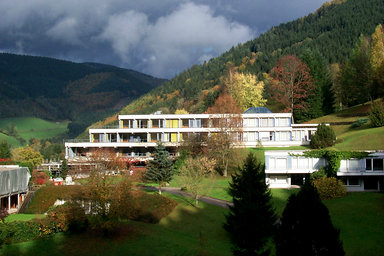
\includegraphics[width=3cm]{photo_mfo.jpg}\\
Das Programm SURFER ist kostenlos auf unserer Homepage erhältlich: \\
\begin{centering}
www.imaginary-exhibition.com\\
\end{centering}
 \vspace{0.2cm}
Sie können rechts die mathematischen Einführungen auswählen, die mit der Zitrus-Fläche beginnen. Links können Sie auf eine andere Galerie springen, z.B. die Galerie der phantasievollen Flächen.
\end{surferIntroPage}